\section*{Figures}

Each figure is also supplied as a separate file at 800~dpi, named by figure number.

\begin{figure}[p]
\centering
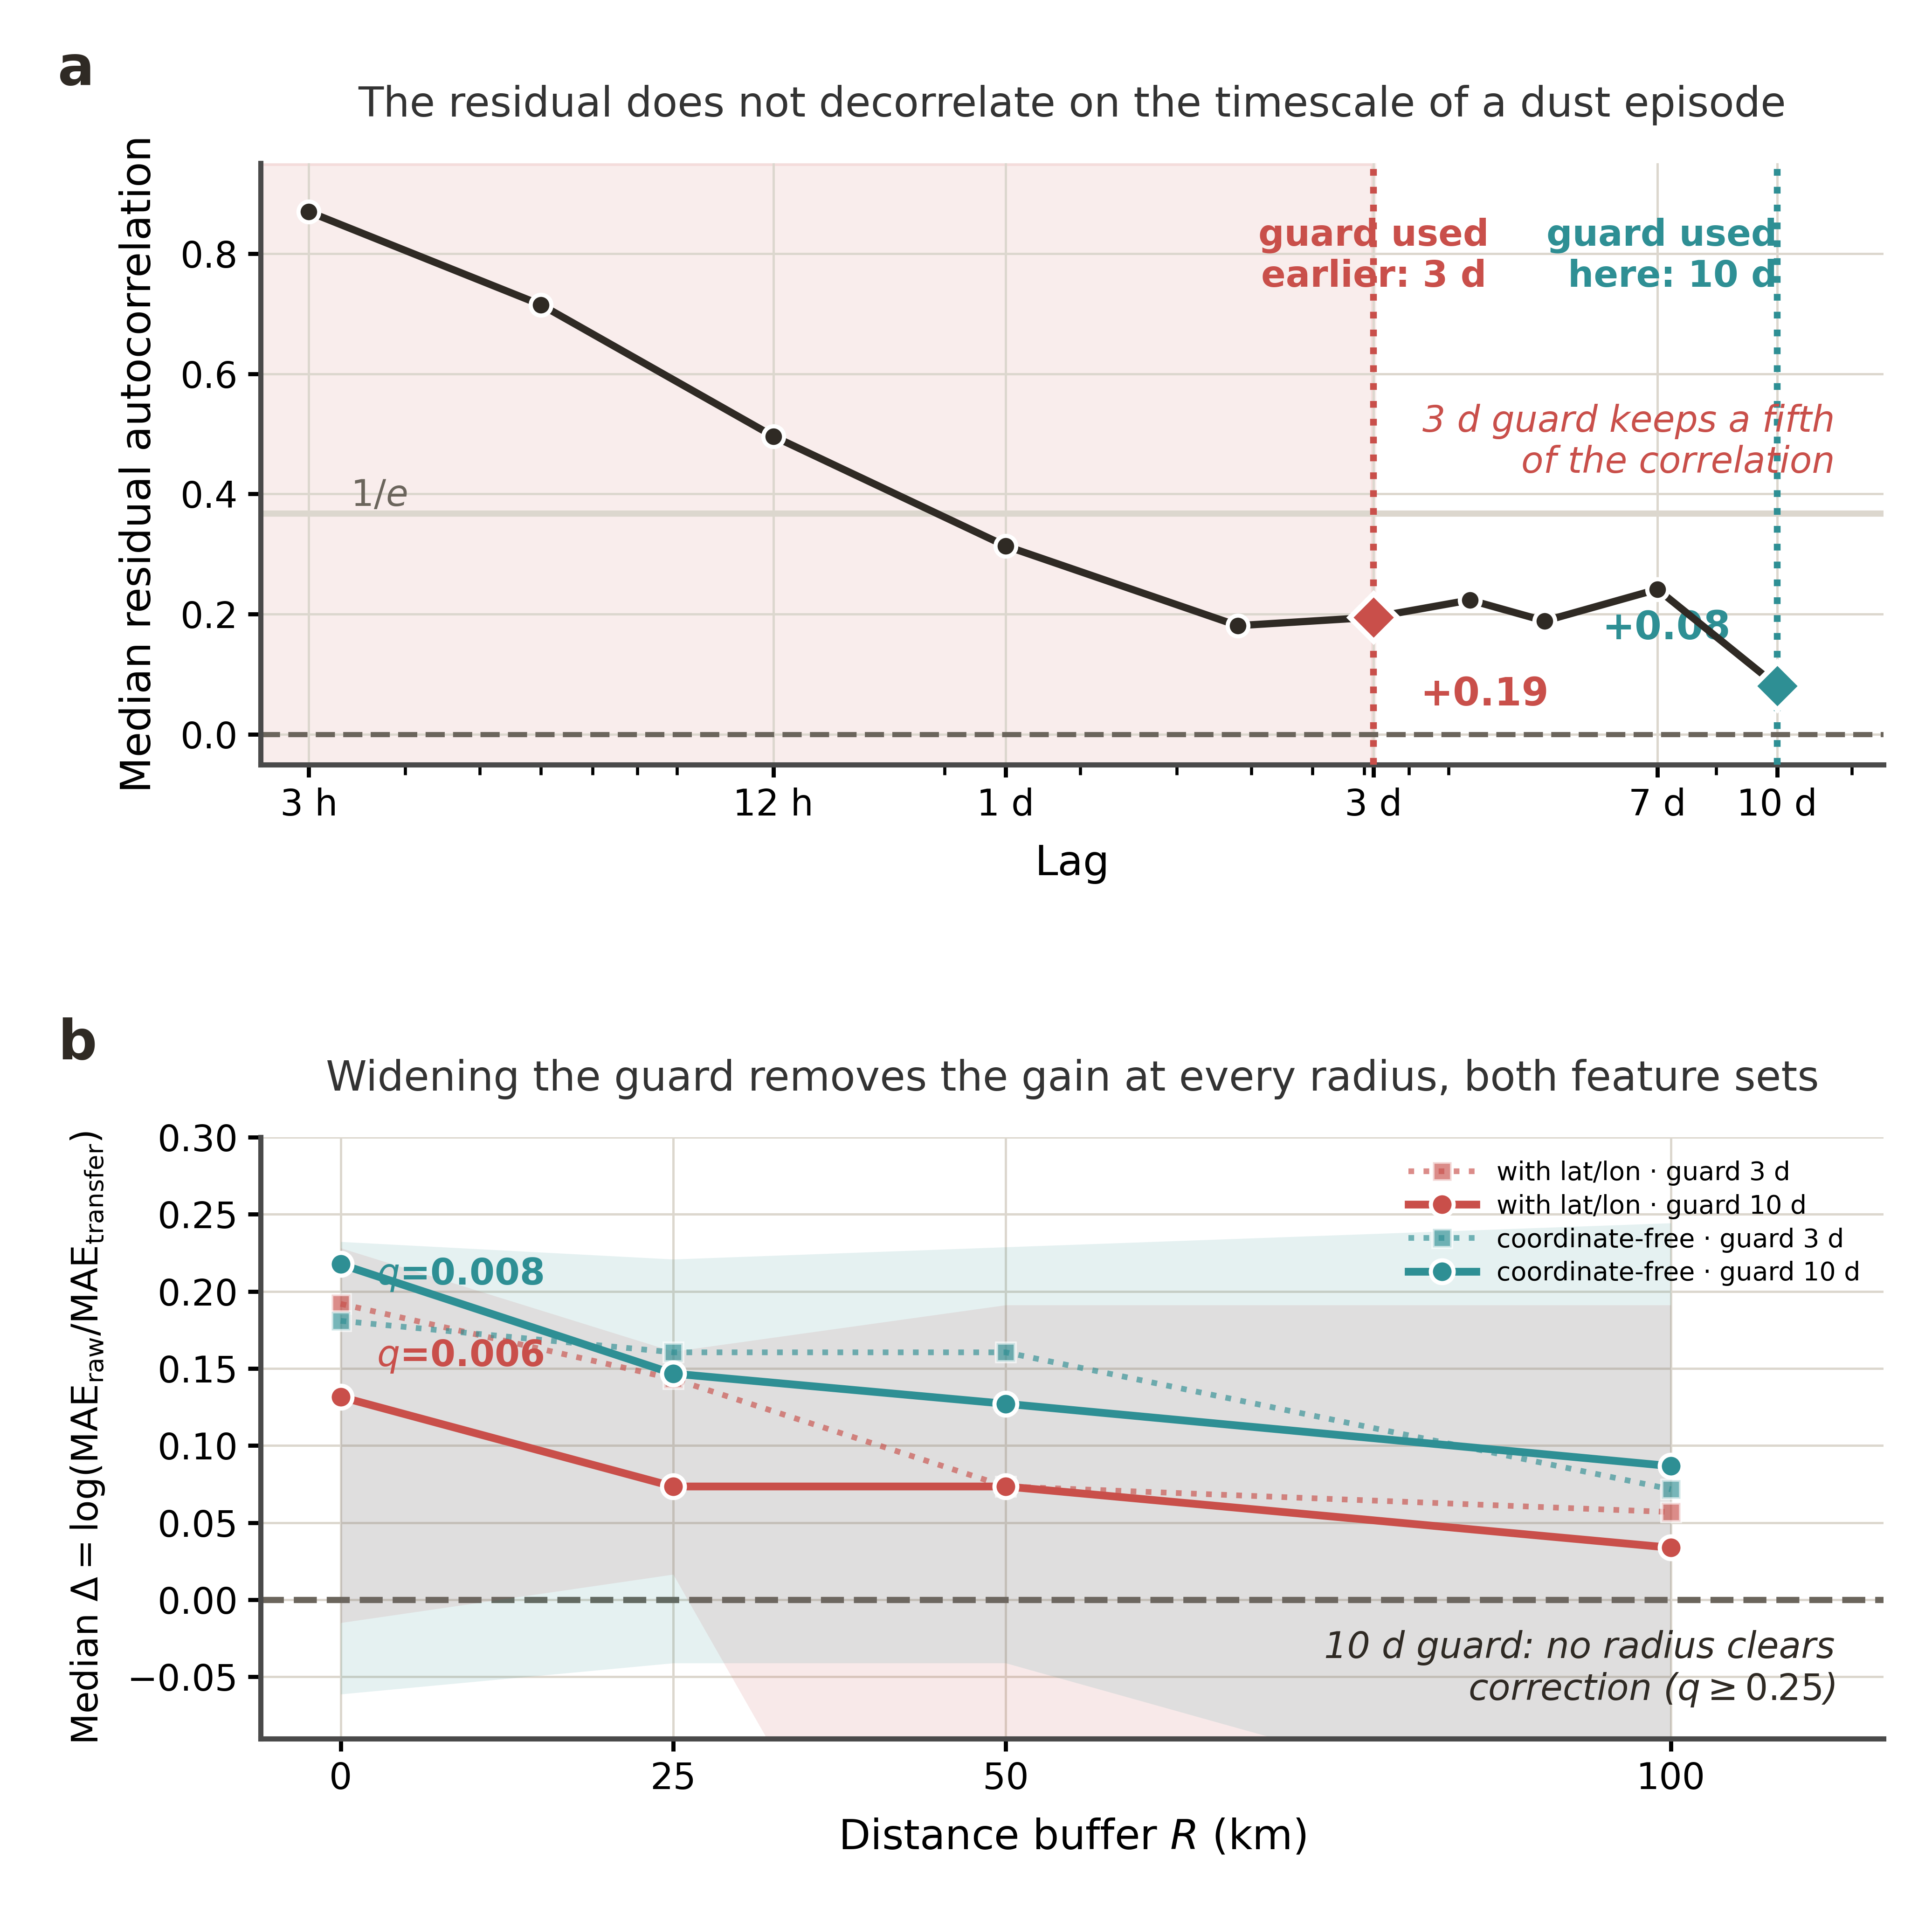
\includegraphics[width=\textwidth]{figures/Empirical_Guard.png}
\caption{The two measured quantities that set the temporal guard.
(a)~Median station-level autocorrelation of the observation-minus-CAMS residual by lag. The
residual is still $+0.19$ at three days and reaches $+0.08$ only at ten days, so a guard taken
from the duration of a dust episode leaves a fifth of the correlation inside the training
window. (b)~Median transfer estimand $\Delta=\log(\mathrm{MAE_{raw}/MAE_{transfer}})$ against
buffer radius for both feature sets under the three-day and the ten-day guard; shading is the
grid-cell block bootstrap. Under the measured ten-day guard no radius clears correction after
Benjamini--Hochberg adjustment ($q\ge0.25$).}
\label{fig:guard}
\end{figure}

\begin{figure}[p]
\centering
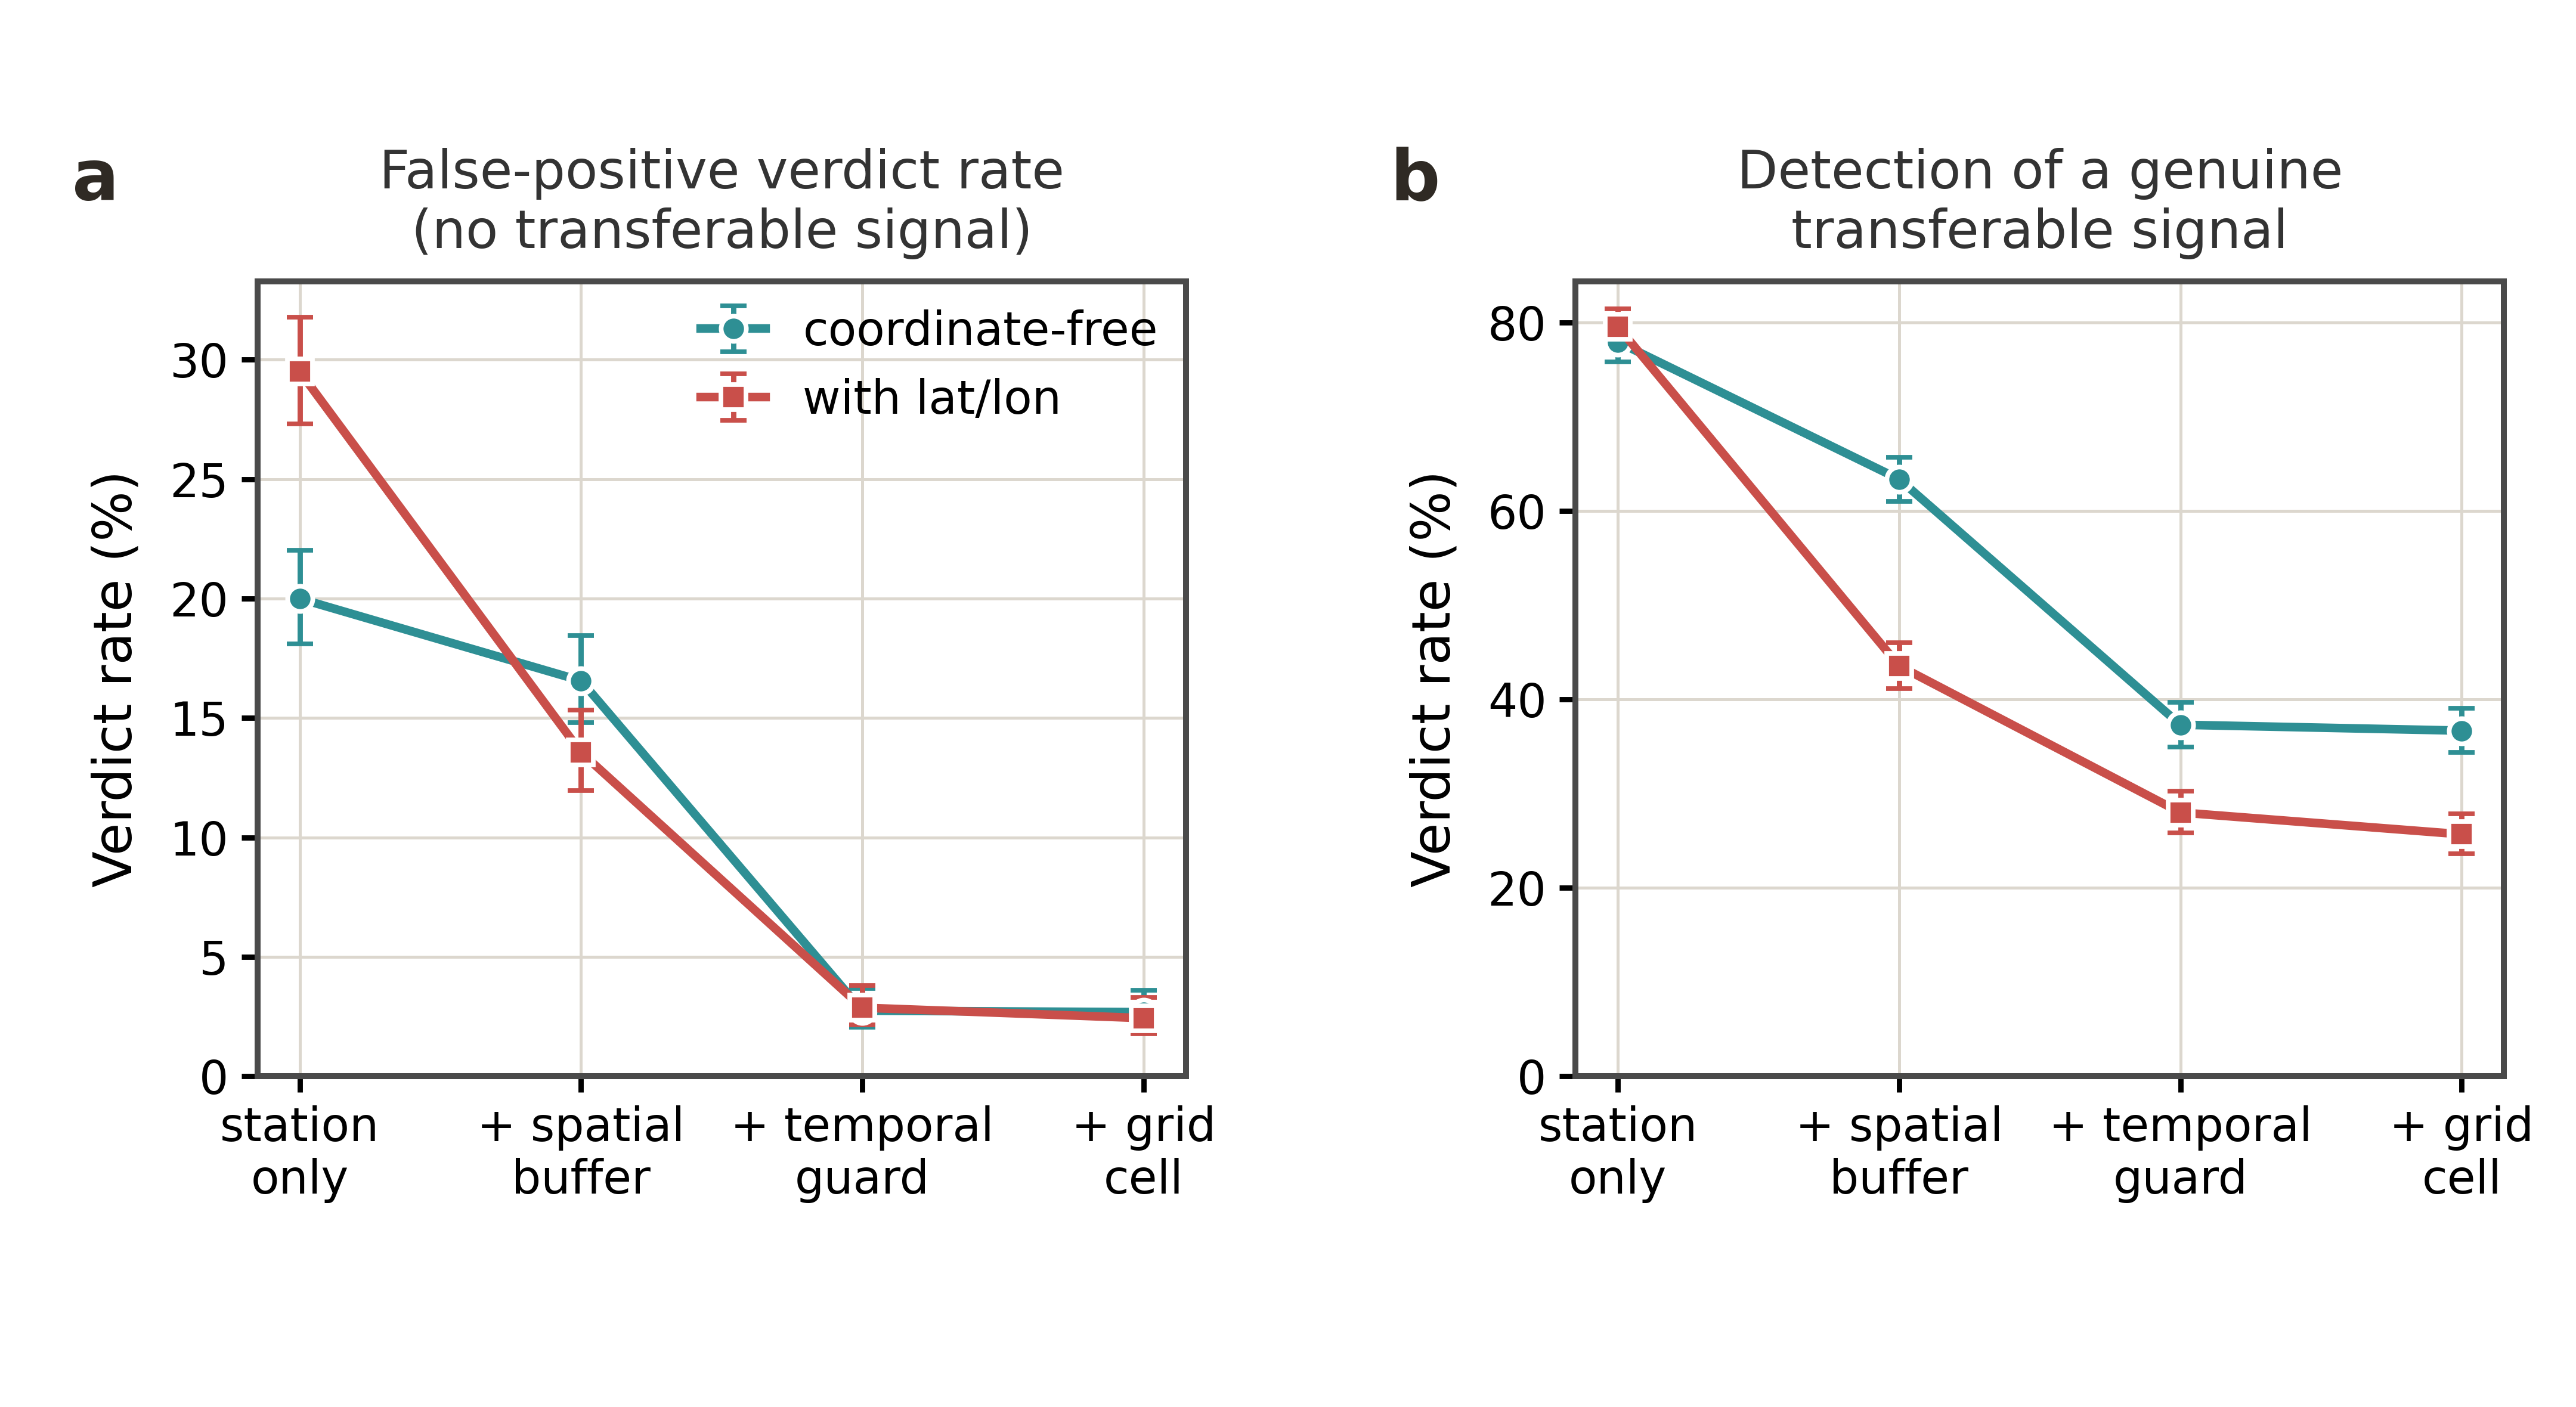
\includegraphics[width=\textwidth]{figures/Simulation_Ladder.png}
\caption{Ground-truth stochastic experiment across the validation ladder, at the primary
$R=50$~km buffer. (a)~False-positive verdict rate when no transferable signal is present.
(b)~Detection of a genuine transferable signal. Bars are Wilson score intervals on the
verdict counts; each point aggregates the pre-declared 32-scenario factorial experiment over
the dependence combinations and the two network geometries. Progressive spatial and temporal
separation sharply reduces false transfer but also reduces detection.}
\label{fig:simladder}
\end{figure}

\begin{figure}[p]
\centering
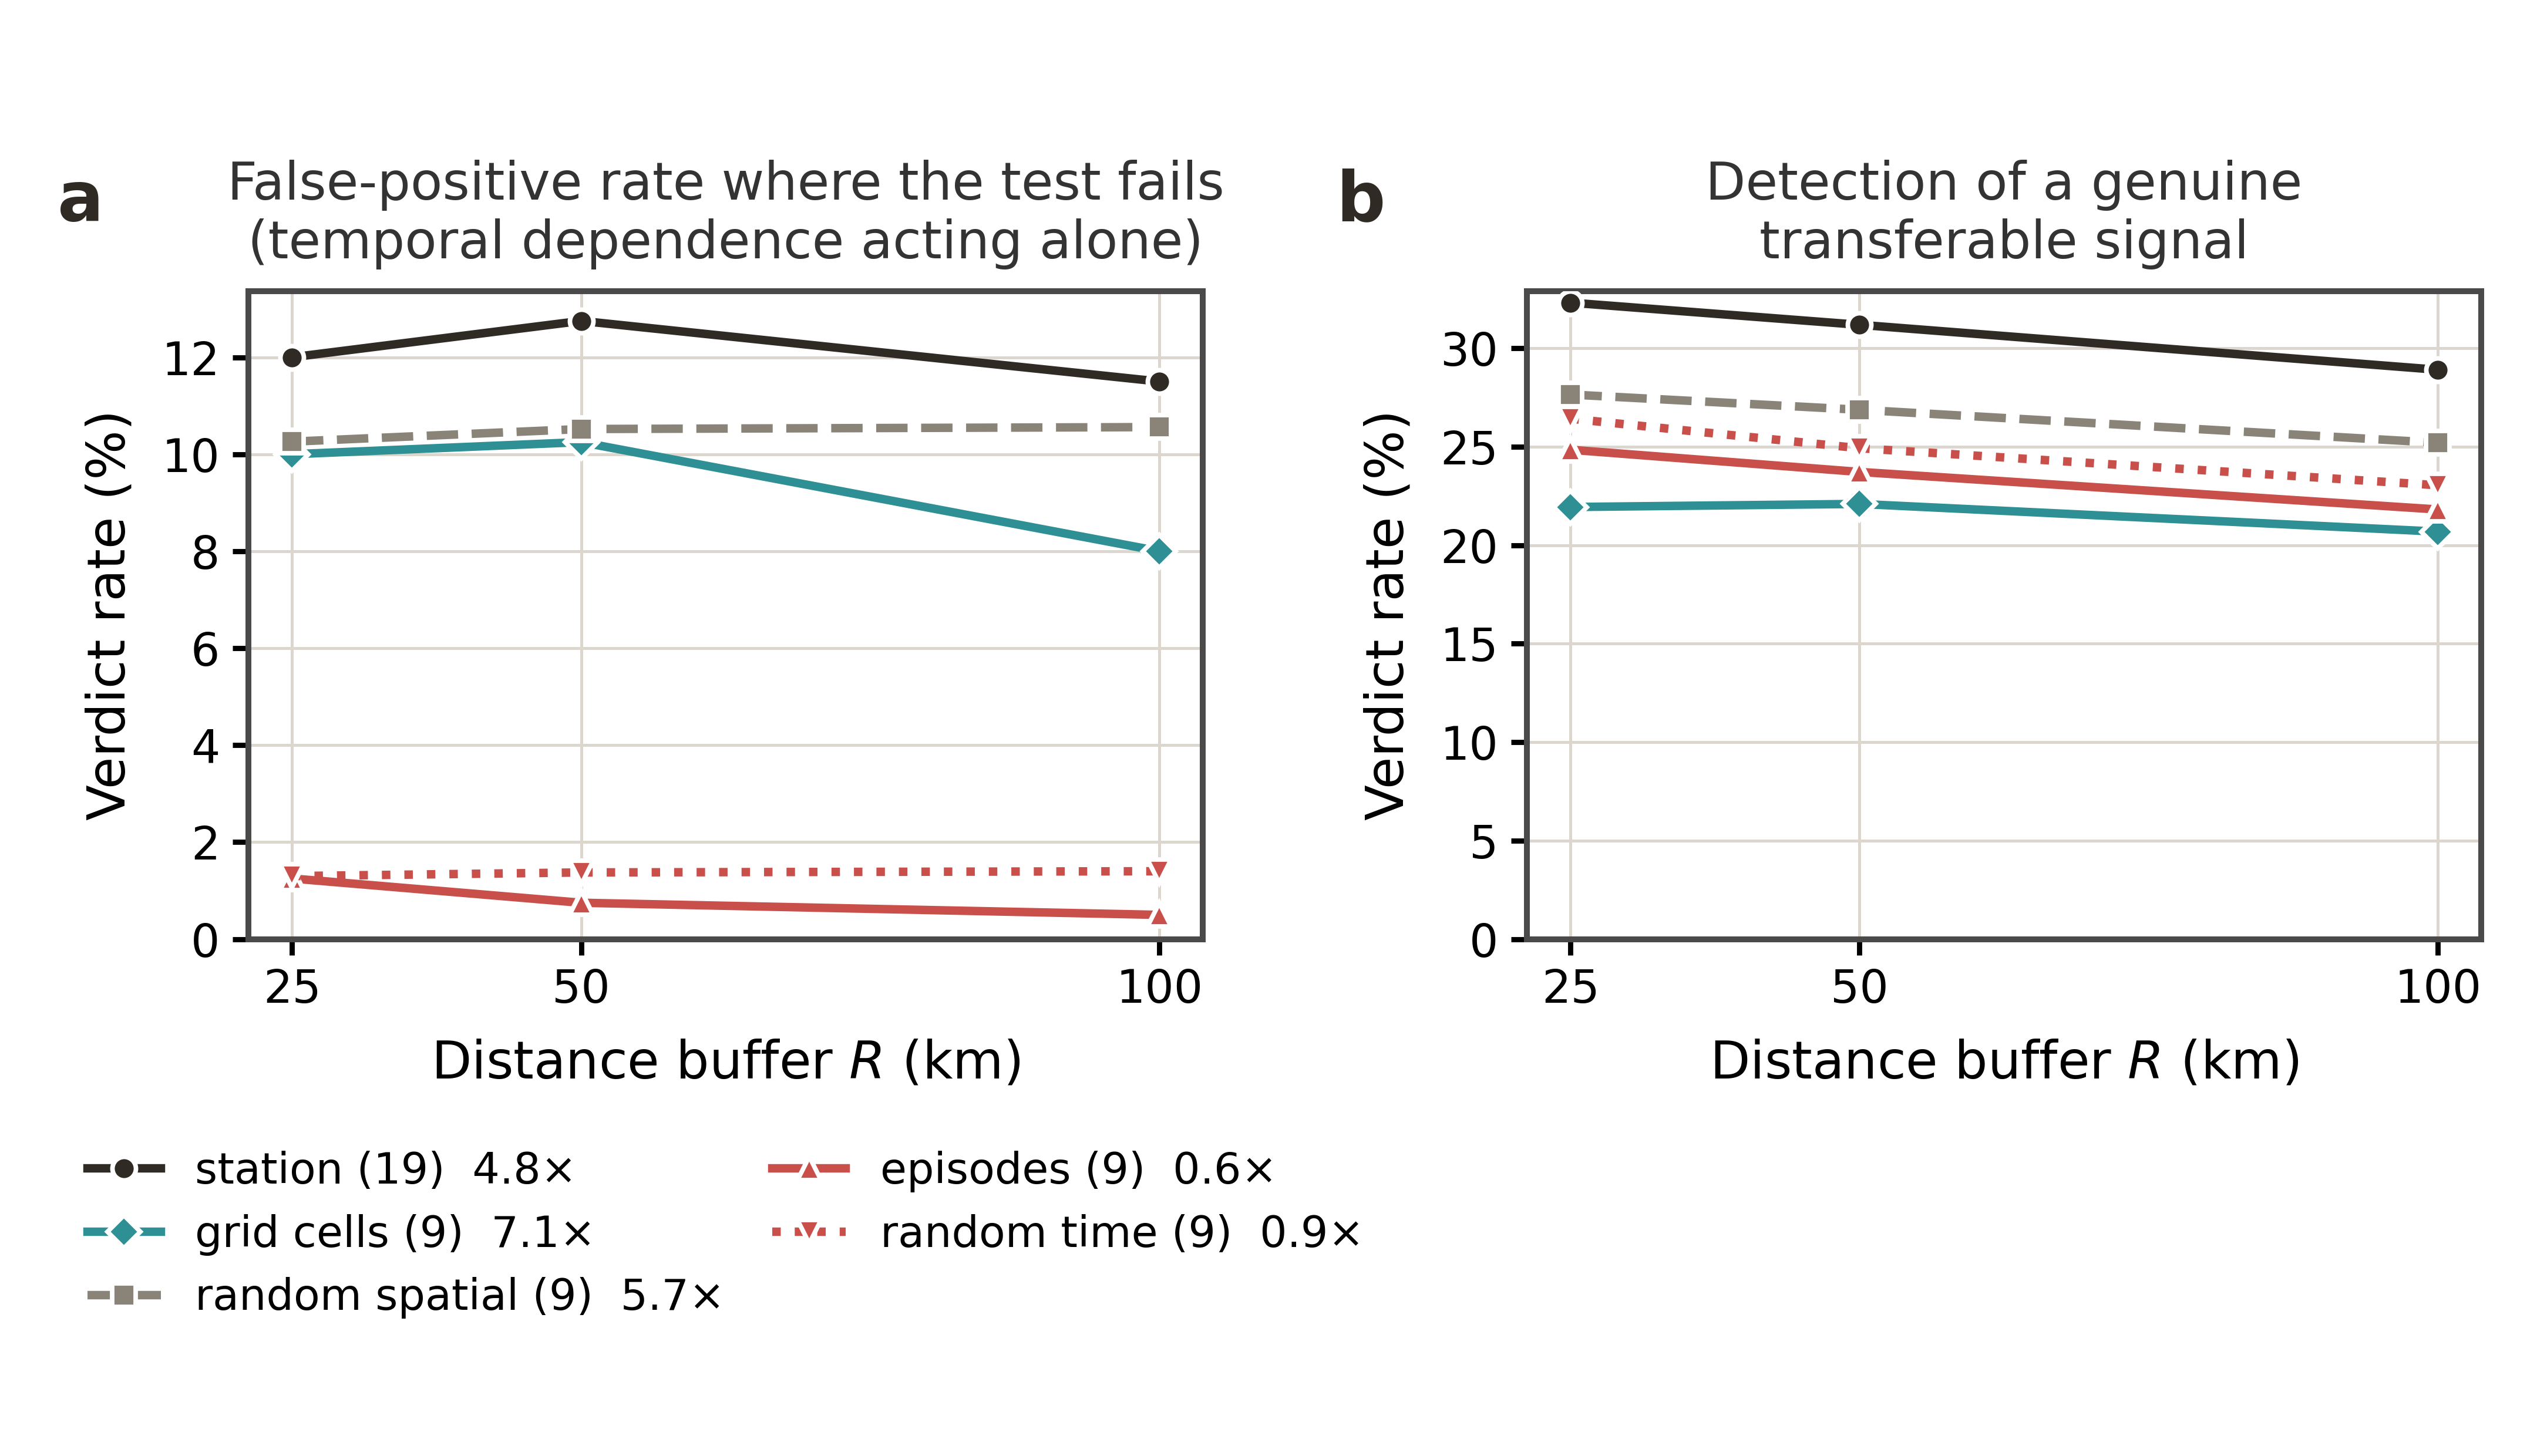
\includegraphics[width=\textwidth]{figures/Unit_Control.png}
\caption{Which inference unit removes the failure, and what it costs. The verdict is a one-sided
exact sign test across held-out units; all five rules are applied to the same realizations, so they
are paired. The station rule counts nineteen targets; the geographic rule the nine occupied
mechanistic-grid cells; the contiguous-episode rule cuts the evaluation window into nine
consecutive blocks; and the two random rules hold the count at nine while destroying the structure
the corresponding structured rule claims to use, averaged over fifty partitions per realization.
(a)~False-positive verdict rate in the corner where the station-level test is anti-conservative:
a residual component common to the network in time, with neither spatial proximity nor shared grid
support. The figure beside each label is that rule's corner rate divided by its own pooled
false-positive rate, which distinguishes a rule that is calibrated here from one that merely
declares transfer less often everywhere; the spatial rules sit between $4.8$ and $7.1$, the
temporal rules at $0.6$ and $0.9$. (b)~Detection of a genuine transferable signal, pooled over the
sixteen scenarios in which one is present. The episode rule costs less detection than the
geographic unit at every radius.}
\label{fig:unitcontrol}
\end{figure}
